\documentclass[a4paper,12pt]{ctexart}     %页面大小和字体大小

\usepackage{ctex}
\usepackage{mathptmx}
\usepackage{amsmath}

\usepackage{url}  % 添加网页

\usepackage{listings}  %添加代码
% 设置代码格式
\usepackage{xcolor}
\lstset{
	language=R,
	backgroundcolor=\color{white}, 
	numbers=left, 
	numberstyle= \tiny, 
	keywordstyle= \color{ blue!70},
	commentstyle= \color{red!50!green!50!blue!50}, 
	%	frame=shadowbox, % 阴影效果
	rulesepcolor= \color{ red!20!green!20!blue!20} ,
	escapeinside=``, % 英文分号中可写入中文
	xleftmargin=2em,xrightmargin=2em, aboveskip=1em,
	framexleftmargin=2em
} 

\usepackage{graphicx} %插入图片的宏包
\usepackage{float} %设置图片浮动位置的宏包
\usepackage{subfigure} %插入多图时用子图显示的宏包


\usepackage{booktabs}  % 三线表


\usepackage{geometry}
\geometry{left=3.17cm, right=3.17cm, top=2.54cm, bottom=2.54cm}   %页边距

\linespread{1.25}      %设置行距


% 摘要设置  -->设置为4号字
\renewcommand{\abstractname}{\textbf{\songti\zihao{4}摘\quad 要}}
\usepackage{setspace}  %行间距的宏包



% 设置标题
\ctexset{
	section={
		format=\bfseries\zihao{4}\songti
	},
	subsection={
	format=\bfseries\zihao{-4}\songti
	}
}

% 设置目录
\setcounter{tocdepth}{2} %设定目录深度为2,即只显示到二级标题为止

% 设置页码
\usepackage{fancyhdr}
\setcounter{page}{1}  %从第一页开始
\usepackage{lastpage} 
\pagestyle{fancy} % 选用 fancy style % 其余同 plain style
\fancyhf{} % 清空当前设置
%\fancyhead{} %清空所有页眉
\renewcommand{\headrulewidth}{0pt}  %页眉线宽,设为0可以去页眉线
\cfoot{} 
\rfoot{\textbf{\thepage/\pageref{LastPage}}}

% 设置附录
\renewcommand\appendix{\par
	\setcounter{section}{0}
	\setcounter{subsection}{0}
	\gdef\thesection{附录 }%\Alph{section}}
	\gdef\thesubsection{附录\arabic{subsection}.}}


% 设置 表的编号的字体大小	
\usepackage{caption}
\captionsetup{font={small,stretch=1.25},justification=raggedright}


\usepackage{listings}  %添加代码
% 设置代码格式
\RequirePackage{color,xcolor}
% 设置代码的默认样式
\lstset{
	frame=none,% 取消边框
	breaklines=true,% 允许自动断行
	% breakatwhitespace=true,% 使用此命令仅允许在空格处自动断行
	showstringspaces=false,% 不显示字符串中的空格
	basicstyle=\small\ttfamily,% 设置代码基本样式
	flexiblecolumns=true,% 改善字母间距
	keywordstyle=\color{blue},% 设置关键词样式
	stringstyle=\color[rgb]{0.75,0,0.75},% 设置字符串样式
	commentstyle=\songti\color[rgb]{0,0.5,0},% 设置注释样式
	tabsize=4,% 设置制表符缩进
}

% 设置python代码环境
\lstnewenvironment{python}[1][]{
	\lstset{
		language=Python,
		keywordstyle=\color[RGB]{255,119,0},% 设置Keywords样式
		morekeywords={as},% 将特定单词加入Kewords中
		deletekeywords={print},%从 keywords中去除特定单词
		keywordstyle=[2]\color[RGB]{144,0,144},% 设置Builtins样式
		morekeywords=[2]{print},% 将特定单词加入Builtins中
		stringstyle=\color[RGB]{0,170,0},% 设置字符串样式
		commentstyle=\songti\color[RGB]{221,0,0},% 设置注释样式	
		#1
	}
}{}




\begin{document}\songti\zihao{-4}
	
	
	
	{\zihao{-2}\heiti
		\title{(选)应用随机过程课程论文\vspace{-4em}}
		\date{}
		\maketitle
	}

	\thispagestyle{fancy} %单独页的页码设置
	
	\begin{center}
		课程号:754.007.201 \quad 时间:2020-2021学年第二学期
	\end{center}
	\vspace*{3\baselineskip}
	\begin{center}\songti\zihao{-2}
		\textbf{隐式马尔科夫模型(HMM)原理介绍}
	\end{center}
	
	\begin{center}
		华光辉 \quad 经济统计1901 \quad 17066003
	\end{center}

	\vspace*{2\baselineskip}   %空白间距


	\begin{spacing}{1.25}

	\begin{abstract}
		隐马尔可夫模型背后的数学是由LEBaum和他的同事开发的。它与早期由RuslanL.Stratonovich提出的最优非线性滤波问题息息相关。在简单的马尔可夫模型(如马尔可夫链),所述状态是直接可见的观察者,因此状态转移概率是唯一的参数。在隐马尔可夫模型中,状态是不直接可见的,但输出依赖于该状态下,是可见的。每个状态通过可能的输出记号有了可能的概率分布。因此,通过一个HMM产生标记序列提供了有关状态的一些序列的信息。隐马尔可夫模型作为一种统计分析模型,创立于20世纪70年代。80年代得到了传播和发展,成为信号处理的一个重要方向,现已成功地用于生物信息学,语音识别,行为识别,文字识别以及故障诊断等领域。也是如今热门的机器学习领域的一个基础模型之一。
		本文通过一个具体实例介绍隐马尔可夫模型,然后介绍该模型中的三个基本问题,以及解决三个问题的方法以及原理
		
		\vspace*{1\baselineskip}   %空白间距
		\noindent{\textbf{关键词:}隐马尔可夫模型,前向后向算法 ,EM算法, 维比特算法 }
	\end{abstract}
	\end{spacing}

	
	
	\section{问题与背景}
	
	\subsection{问题}
	本文采用李航老师《统计学习方法》一文中的例子,
	
	转移概率矩阵
	
	\begin{table}[htbp]\songti\zihao{5} 
		\begin{center}
			\renewcommand\arraystretch{2}         %表格内部 1.5 倍行距离
			\caption{模型数据 \label{tab:hezi}} 
			{\tabcolsep0.3in  %设置列间距
		
				\begin{tabular}{|c|c|c|c|c|}\hline   %开始表格环境,{|c|c|c|}表示文字居中的三列,\hline...\hline表述画两条并排的水平线。
					%\hline必须用于首行之前或者换行命令之后。
					
					\small 盒子编号&1&2&3&4\\\hline   %&是数据分割符号
					红球数&5&3&6&8\\\hline
					白球数&5&7&4&2\\\hline
				\end{tabular}
			}
		\end{center}
	\end{table}
	
	
	
	观测概率矩阵
	
\begin{table}[htbp]\songti\zihao{5} 
	
	\begin{center}
		\renewcommand\arraystretch{2}         %表格内部 1.5 倍行距离
		\caption{观测概率矩阵 \label{tab:shuoming}} 
		{\tabcolsep0.3in
			
			\begin{tabular}{|c|c|c|}\hline   %开始表格环境,{|c|c|c|}表示文字居中的三列,\hline...\hline表述画两条并排的水平线。
				%\hline必须用于首行之前或者换行命令之后。
				
				\small &$ v_1 $&$ v_2$\\\hline   %&是数据分割符号
				$ q_1 $&0.5&0.5\\\hline
				$ q_2 $&0.3&0.7\\\hline
				$ q_3 $&0.6&0.4\\\hline
				$ q_4 $&0.8&0.2\\\hline
			\end{tabular}
		}
	\end{center}
\end{table}
	转移概率矩阵
	\begin{table}[htbp]\songti\zihao{5} 
		\begin{center}
			\renewcommand\arraystretch{2}         %表格内部 1.5 倍行距离
			\caption{模型数据 \label{tab:hezi}} 
			{\tabcolsep0.3in  %设置列间距
				
				\begin{tabular}{|c|c|c|c|c|}\hline   %开始表格环境,{|c|c|c|}表示文字居中的三列,\hline...\hline表述画两条并排的水平线。
					%\hline必须用于首行之前或者换行命令之后。
					
					\small &$ q_1 $ &$ q_2 $&$ q_3 $&$ q_4 $\\\hline   %&是数据分割符号
					$ q_1 $&0&1&0&0\\\hline
					$ q_2 $&0.4&0&0.6&0\\\hline
					$ q_3 $&0&0.4&0&0.6\\\hline
					$ q_4 $&0&0&0.5&0.5\\\hline
				\end{tabular}
			}
		\end{center}
	\end{table}
	
	\subsection{符号解释}
	隐马尔可夫模型中的三个基本问题
	
	\begin{table}[htbp]\songti\zihao{5} 
		
		\begin{center}
			\renewcommand\arraystretch{1.5}         %表格内部 1.5 倍行距离
			\caption{符号说明 \label{tab:shuoming}} 
		{\tabcolsep0.25in   % 设置列间距
			\begin{tabular}{ll}
				\toprule    
				属性 & 符号  \\    
				\midrule 
				所有可能状态的个数 &$ N $ \\
				所有可能观测的个数 & $ M $ \\ 
				状态序列的个数 & $ T $  \\   
				单次状态 & $q_i$ \\ 
				所有可能状态的集合 & $ Q = \{ q_1,q_2,\dots,q_N\} $  \\
				单次观测 & $ v_i $  \\ 
				所有可能观测的集合 & $ V = \{ v_1,v_2,\dots,v_M\} $  \\
				状态序列 & $ I = \{i_1,i_2,\dots,i_T\} $  \\
				观测序列 & $ O = \{ o_1,o_2,\dots,o_T\} $ \\
				状态转移概率 & $ a_{ij} = P(i_{t+1} = q_j | i_t = q_i) $ \\
				条件观测概率 & $ b_j(k) = P(o_t = v_k| i_t = q_j)$ \\ 
				状态转移矩阵 & $ A = [a_{ij} ]_{N \times N} $ \\
				观测矩阵 & $ B = [b_j(k)]_{N \times M} $ \\
				初始状态概率 & $ \pi_i = P(i_1 = q_i)$ \\
				初始状态概率向量 & $ \pi = (\pi_i) $ \\
				所有参数 & $ \lambda = (A,B,\pi) $\\  
				\bottomrule   
				
			\end{tabular} 
		}
		
		\end{center}
	\end{table}
	








		\begin{figure}[H] %H为当前位置,!htb为忽略美学标准,htbp为浮动图形
		\centering %图片居中
		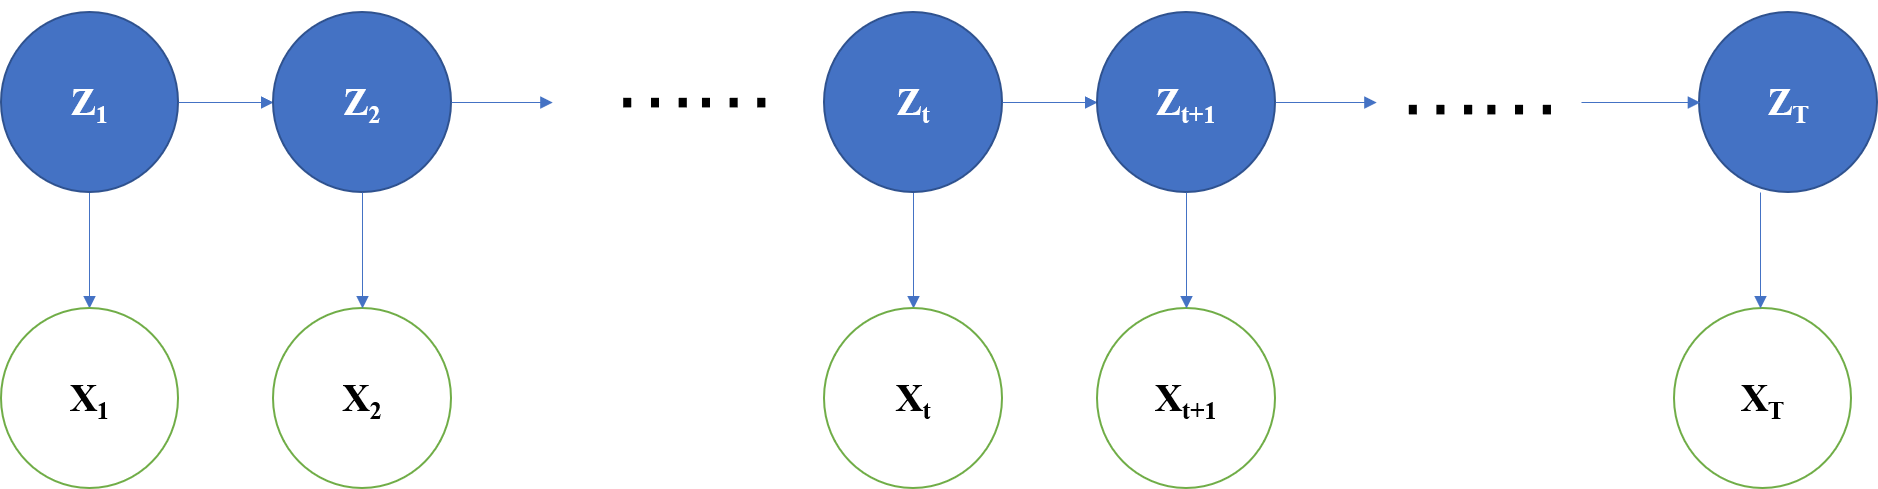
\includegraphics[width=0.7\textwidth]{示意图.png} %插入图片,[]中设置图片大小,{}中是图片文件名
		\caption{示意图 \label{shiyitu}} %最终文档中希望显示的图片标题
		\end{figure}
	

	\begin{thebibliography}{99}    %参考文献开始
		\bibitem{1}李航,统计学习方法,北京:清华大学出版社,2012.3。     
		\bibitem{quanjing} Weisong Zhao,HMM隐马尔可夫模型详解,\url{https://blog.csdn.net/weixin_41923961/article/details/82750687},20(3),2021。
		
		
		
		
	\end{thebibliography}

	
	\addcontentsline{toc}{section}{参考文献}
	
	
	
	\begin{appendix}

	\begin{center}
		\section{}
	\end{center}

	\subsection{原始数据}
	\subsection{随机模拟程序及运行结果}
	\begin{python}
import numpy as np
pi = np.array([.25, .25, .25, .25])
A = np.array([
[0,  1,  0, 0],
[.4, 0, .6, 0],
[0, .4, 0, .6],
[0, 0, .5, .5]])
B = np.array([
[.5, .5],
[.3, .7],
[.6, .4],
[.8, .2]])

def get_data_with_dist(dist):
	r = np.random.rand()
	print(r)
	for i, p in enumerate(dist):
	if r < p: return i
	r -= p

def generate(T: int):
	z = get_data_with_dist(pi)    
	x = get_data_with_dist(B[z])  
	result = [x]
	for _ in range(T-1):        
	z = get_data_with_dist(A[z])
	x = get_data_with_dist(B[z])
	result.append(x)
	return result

generate(3)
		
		\end{python}
	
	\end{appendix}

\end{document}
